
\section{How to Analyze Usage Data}

When collecting usage data it is imporant to have the end in mind. How will this data be used to address the research question at hand? Not surprisingly, the nature of the collected data, especially whether it is anonymous, dramatically effects what can be learned.


\subsection{Types of Data}

\noindent
{\bf Non-anonymous data}, where sensitive information including source code snippets, change-sets, and even access to the source code base is provided has obvious advantages. Researchers can replay developers' activity stream, affording them a deep understanding of the developer's actions~\cite{UseDisuseMisuseRefactoringsExtendedVersion}. There are few limits on how this data can be analyzed, and {\em non-anonymous data is well-suited for exploratory studies}. Unfortunately, there are some key disadvantages. First, only developers working on open source systems are likely to participate in such studies; typical enterprise developers may face termination if they were to leak even parts of their source code base. Second, while playback and other deep analyses are possible, these analyses can be costly in terms of time and resources. 

\vspace{0.1in}

\noindent
{\bf Anonymous data}, where only records of activities and anonymous facts about artifacts are recorded, may at first seem strictly inferior. Indeed there are some limitations on what can be learned from anonymous activity streams, yet there are key advantages. First, developers are receptive to data collection for research purposes, and thus the ability to collect a large amount of information from many developers increases greatly. Second, because the data set is relatively large and is harvested from working developers, conclusions are ultimately more reliable. 

In this section we focus on analyzing anonymous data sources. We do so because analyzing anonymous activity streams is similar to analyzing non-anonymous data streams (i.e., they are both activity streams) and because the unlimited variation of analysis permitted by non-anonymous data affords few generalities. As we discuss analyzing usage data we start with straightforward magnitude analysis, build to a categorization system for activity streams, discuss dividing streams into sessions, and finally state-based analysis. 


\subsection{Usage Data Format}
Most usage data is collected as an activity stream with varying levels of supporting detail. In Figure~\ref{fig:theoretical} we present an abstraction of a typical activity stream. It includes a time-stamp, followed by the activity, appended with (often anonymous) details concerning that activity. We can apply this model to the examples discussed earlier. For instance, the Mylyn Monitor's interaction event corresponds to a row in our theoretical model. It includes a time-stamp (i.e., StartDate), an activity description (i.e., Kind, OriginId), and additional information (i.e., StructureHandle, StructureKind). Similarly, the CodingSpectator example includes a time-stamp (i.e., stamp), an activity description (i.e., id), and a much larger set of additional information (i.e., code-snippet, selection, selection-in-code-snippet, etc.). Because these and other usage data activity streams can easily be described using our abstraction we will refer to it as we describe data analysis techniques.


%TODO: Rewrite/Adapt/Remove this paragraph now that it's been integrated

%What do they look like

%include theoretical example

%several concrete examples (codingsepctator, Sando, Eclipse study)

%Software systems often keep a record about what event was completed (or not) in the form of a log file. The information collected in the log file is often used for diagnostic purposes. If a system failure occurs, the logs for that period can be inspected to see which sequence of events were executed by the system and what were the values for the dynamic information in those events. Each log line can be traced back to a particular line of code where the method to log this information was called. Hene, we can get complete information on what events were executed. The log message store information about the branches taken by that particular instance of execution and the values for variables in the code. Due to these reasons, the information in the log file is collected as a serially ordered flat text file. In short, a log file is a collection of log lines, with each of them having information about a single event, its time of execution and the dynamic information about variable values. Note that each log line may span across multiple lines, but provides information to distinct two adjacent log lines.



\begin{figure*}[t]
 \centering
\includegraphics[width=1\columnwidth]{activityLogTheoretical.pdf}
\caption{Abstract model of developer activity streams.}
\label{fig:theoretical}
\end{figure*}



%\begin{figure*}[t]
 %\centering
%\includegraphics[width=0.5\columnwidth]{activityEvent}
%\caption{Activities as Captured in an Eclipse Usage Data Study}
%\label{fig:activity}
%\end{figure*}
%
%\begin{figure*}[t]
 %\centering
%\includegraphics[width=0.5\columnwidth]{codingSpectator}
%\caption{Activities as Captured in a CodingSpectator Study of Refactoring Events}
%\label{fig:activit}
%\end{figure*}



\subsection{Magnitude Analysis}
%advantages
A major advantage of anonymous usage data is the fact that it captures developers in their natural habitat, without any observational bias. Deriving conclusions from hours of developers' field work is naturally more convincing than from hour-long, in-lab user studies. One type of questions that usage data is well-suited to answer uses measurement of the magnitude of occurence of a specific event. For instance, researchers may want to know ``How often do developers invoke the pull-up refactoring'' or ``How often is the file search invoked?''. By performing a count of a specific message in the collected logs, researchers can easily calculate frequencies of specific actions that can be often sufficient to answer important research questions. 

%disadvantages
However, researchers must be wary of a few common issues with magnitude analysis. First, in any sufficiently large set of user logs there is a small set of users that will use the feature/tool under analysis orders of magnitude more often than the general population, potentially skewing the data. Second, any fine-grained attempt to qualify the raw counts requires making possibly incorrect assumptions about the data. For instance, there is a temptation to report refactorings per hour, yet any fine-grained time calculation requires assumptions about how time was spent between activities, which experience has taught us are often wrong. Note that coarse-grained qualification, such as refactorings performed per day, are possible.   

%example
\begin{figure}
  \centering
  \includegraphics{AnalyzingUsageData/eclipse}
  \caption{Breakdown of Navigation-Focused View Usage in Eclipse}\label{fig:eclipse}
\end{figure}




\subsection{Categorization Analysis}
Magnitude analysis is well-suited for analyzing low-level behavior, yet most research questions are at a higher level. The research question ``How often are refactorings performed?'' cannot be answered via magnitude analysis alone, as refactorings can be triggered through tens of different commands. These commands first need to be categorized, after which magnitude analysis can be used. When focusing on a concrete sub-task, such as refactoring, it may be easy to categorize activities. In this case, all refactoring commands, such as pull-up or extract method, can be classified as refactorings. However, when focusing on more general behavior, such as editing, navigating, and searching, categorizations can be difficult. It is impossible to say, for instance, from a single click in the file explorer whether that click represents a search, as the developers browses a few promising files, or a navigation, as he implicitly opens a type declaration of a variable he was just browsing. Thus, categorization at the individual action level is necessarily noisey data, which effects the strength of conclusions that can be made from it.

\begin{figure*}[t]
 \centering
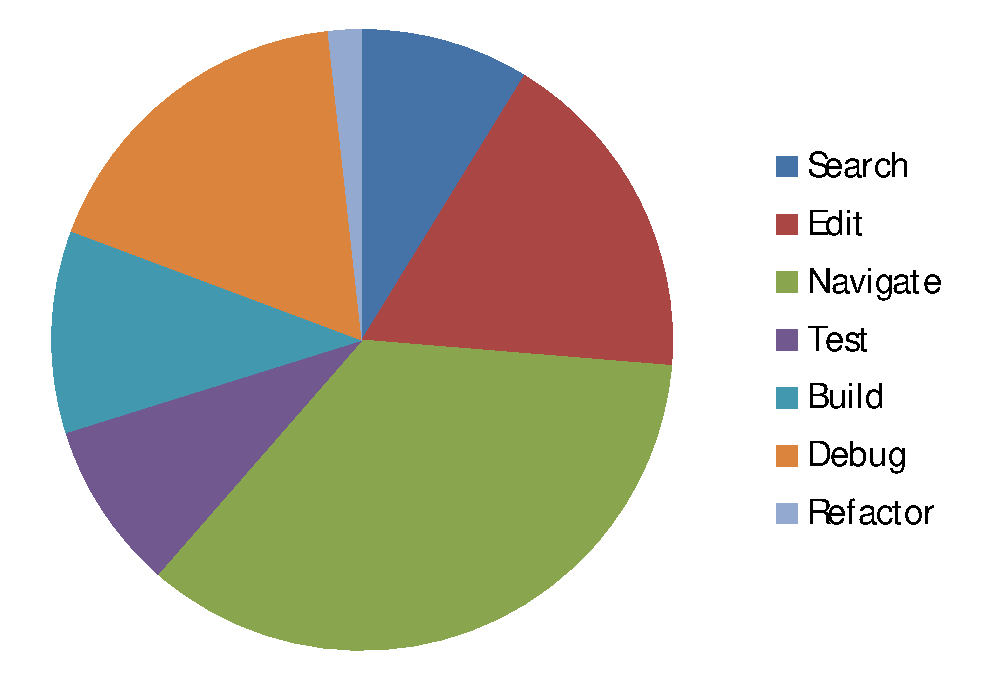
\includegraphics[width=0.5\columnwidth]{../Graphics/activityCategorization.pdf}
%\caption{Pairwise matches across categories, including matching and mismatching pairs.}
\label{fig:category}
\end{figure*}

\subsection{Sequence Analysis}
%intro to seqence analysis, sessions
Magnitude analysis and categorization are both appropriate for answering simple research questions. However, a more powerful way of analyzing activity logs is through sequence analysis, which first breaks activity sequences into session, according to some criteria, and then reports upon characteristics of that session. A session is a particular interaction with an IDE by a specific user in order to complete a task (e.g. refactoring, looking for a starting point for a maintenance task, etc.), consisting of all of IDE events in a given time span.
For instance, answering the research question of ``Are developers successful at finding initial points in the code for a software maintenance task?'' requires that the sequence of IDE events corresponding to each maintenance task be identified, before we can perform further analysis using either magnitude or categorization analysis. The granularity of a session is determined by the guiding research question. For certain research questions, we may be interested in a smaller session (e.g. searching the code base), while for others we may need to consider a longer time span (e.g. performing a maintenance task, developing a new feature). 

%how difficult or easy is it to determine sessions
In many cases, extracting sessions from activity sequences can be challenging as it impossible to know exactly when a developer begins or ends a particular task, without understanding his or her underlying thought process. There are several possibilities in how session extraction can be performed, based on the task related to the specific research question. One possibility is to use sentinels, which are specific actions where we can detect a task begins or ends. For instance, in code search, submitting a query to the code searcht tool begin one task and end the prior task in the activity stream. Another possibility is to use the passage of time to extract sessions, where time without any activity is used as a signal of task start or finish. Coman et al.'s \cite{Coman-TaskIdent} algorithm uses a combination of key events in the activity stream and time distance between such events to extract relevant sessions corresponding to developer tasks. In lab validation studies this algorithm has shown very high accuracy (80\%) when compared to the ground truth reported by developers, however this accuracy may not hold up in an industrial setting\cite{Zou-ComanIndustry}.


%example
As an example of sequnce analysis, consider a researcher investigating finding initial points in the code for a software maintenance task. Specifically, the developer is interested in the following research question ``Are users satisfied with file search results?''. This question, while impossible to answer via simple magnitude analysis can be investigated via session analysis. Using assumptions from in-lab studies that show that opening a search result followed by a long pause correlates with user satisfaction we can analyze activitiy logs to determine how often user behavior indicated satisfaction in the field. The researcher may break activity logs into sessions, starting with a search being executed and ending on the last interaction with that result set. He could calculate additional characteristics from this raw data, such as the amount of time spent per session, the number of results reviewed, and the number of files opened.   


\begin{figure*}[t]
 \centering
\includegraphics[width=1\columnwidth]{../Graphics/activityLogActual.pdf}
%\caption{Pairwise matches across categories, including matching and mismatching pairs.}
\label{fig:actual}
\end{figure*}

%Sequence analysis is currently the most powerful tool we have for analyzing logs. While there has been preliminary work to complete annotate activity logs into tasks or even states (e.g., editing, searching, navigating, testing, etc.) these analyses are currently unreliable. In fact, we believe that because user behavior is often multi-purposed there will remain major obstacles to inferring higher-level user states from activity streams, ultimately limiting the usefulness of any full log analysis. 




\subsection{State Model Analysis}
As the number of data points increases, it is difficult to perform menaingful analysis using the methods mentioned in earlier. In state model analysis, the sequencial data is conveted to nodes and edges of a graph which represents the enrire data and states. Data can be analysed accurately and efficiently by transforming the serially ordered events in a sequence data to a Weighted Directed Graph (WDG) data structure. Only the information needed for the analysis need to be maintained and condensed into a compact view of the log file. We can abstract the information in the log line to any level, such as, event level, method level, class level, file level, sub-module level, or module level. In the sequence data, each event is important as a standalone event. However, in the WDG representation, the importance shifts to adjacent pairs of events. We do this type of a transformation to record the order in which events happened. Therefore, each unique event in the sequence data is represented by a unique node in the WDG. An edge exists from one node (head) to another (tail) if there is an occurrence of the event representing the tail node immediately after the event representing the head node in the original log file. For example if event B follows event A in the log file, then there is directed edge from node A to node B in the WDG. The edges are labeled with the number of times this transition has occurred.  For example if B occurs a fifty times after A in the log file, then the edge from node A to node B in the WDG is labeled with 50. Typically, we keep track of the actual count as the weight of the edge, when building the graph. In the graph we display the percentage value as the label. This percentage is propotional to the total number of transitions.  The cumulative probability of out-edges of a node is 1. The transitional probabilities of each out-edges are calculated by dividing the number of transactions of that out-edge with the sum of all outward transactions from that node. We could also store the dynamic parameter information in each log line as a list along the edges. We now present the steps involved in this transformation. Consider that the input log file is with $N$ log lines. We need to convert this log file WDG.

State model analysis is helpful when the number of data points are more and when there is a repetation of a set of data points. State model provides information about the probability of occurance of each state and the transistional probaility of each activity. This information is helpful for many analysis. 

However, when the number of states are more, the WDG becomes more complex and hence difficult to understand. in such cases, identifying the most active states and edges provides information about the important activities in the data set. This approach is more suitable when the number of states in the data set is less than 30. If the number of states is more, either use some other analysis or combine the states to get more menningful data. (for example, if the data set consists of the interactions of methods in a source code and the number of methods is quite high, it is better to do the analysis at the class level which will be less in muber and provides more insight to the relationships.



To explain the steps with an example, consider a simple log file where the activities are spearated by commas. $1-2, 2-3, 3-4, 4-5, 5-4, 4-5, 5-4, 4-6, 6-7, 7-5, 5-4, 4-5, 5-4, 4-5, 5-8, 8-9$. The events in the log file are mapped to their corresponding event IDs: $1, 2, 3, 4, 5, 4, 5, 4, 6, 7, 5, 4, 5, 4, 5, 8, 9$. Each node is a unique event. An edge between nodes 1 and 2 signifies that the event 2  appears after event 1  in the log file. The labels on the edges have the actual count and could have the transitional probabilities as well. The transitional probability from node 1 to node 2 is 1.0, whereas the transitional probability from node 4 to node 6 is 0.2.  This is depicted in Fig \ref{op-profile-example}.


JUMBL (Java Usage Model Builder Library) developed by Software Quality Research Laboratory (SQRL) of University of Tennessee \cite{jumbl} can be used for developing operational profile and calculating the probability of usage by each state of the operational profile. JUMBL is a collection of tools to support automated, model-based, statistical testing of systems \cite{jug}. JUMBL helps in

\begin{itemize}
\item Constructing usage models from component states
\item Generating tests in various ways
\item Converting tests to executable data to support test automation, and
\item Assessing testing by providing test measures, including expected system reliability in the field.
\end{itemize}

WDG along with the transitional probability are used to determine the state probabilities of each component . We have used JUMBL to create the state probabilities \cite{anil}. We have converted the WDG to JUMBL readable TML \cite{tug} language. We have developed tools, which will mine the log file and convert the log file to an adjacency matrix representation with the number of transitions from each node, which is translated directly to TML script. A sample log file is and the corresponding TML fileare given below. The TML script has information about the nodes, the out edges from each node along with the number of transitions from each node to another. This TML script is used in JUMBL to arrive at the state probabilities of each node. State probabilities give information about the percentage of usage of each node. Corresponding graph is depicted in Fig. \ref{op-profile-example}



\begin{verbatim}
2013-03-21 18:18:32Z,A
2013-03-21 18:18:33Z,B
2013-03-21 18:20:49Z,C
2013-03-21 18:20:50Z,A
2013-03-21 18:20:56Z,B
2013-03-21 18:20:57Z,A
2013-03-21 18:21:08Z,C
2013-03-21 18:21:08Z,D
2013-03-21 18:21:08Z,E
2013-03-21 18:21:08Z,A
\end{verbatim}


\begin{verbatim}
// Usebased model for testlog

($ fill(1) $)
model testlog
//use this before each transition to show probability ($0.10$)

source [A]
($2$)"Count=2 (A->B), TimeElapsed= 7secs" [B]
($1$)"Count=1 (A->C), TimeElapsed= 11secs" [C]

[B]
($1$)"Count=1 (B->C), TimeElapsed= 136secs" [C]
($1$)"Count=1 (B->A), TimeElapsed= 1secs" [A]

[C]
($1$)"Count=1 (C->A), TimeElapsed= 1secs" [A]
($1$)"Count=1 (C->D)" [D]

[D]
($1$)"Count=1 (D->E)" [E]

[E]
($1$)"Count=1 (E->A)" [A]


"exit" [Exit]

end 
\end{verbatim}



\begin{figure}
  \centering
  \includegraphics[scale=.40]{../Graphics/op-profile-example.png}
  \caption{Weighted Directed Graph of the Example Log}\label{op-profile-example}
\end{figure}


A sequence data with hundreds of thousands of lines can be quickly convereted to more meaningful graphical represeantation using this method. Once the TML file is generated, we can use JUMBL to find out the state probabilities of each states. usaing the state probaility and the usage patterns we can arrive conclusions and can visualize them easily like mentioned in figures  \ref{fig:sample_log} and \ref{fig:log_with_color}

\begin{figure}
  \centering
  \includegraphics[scale=.15]{../Graphics/log_with_color.png}
  \caption{WDG example with probability}\label{fig:log_with_color}
\end{figure}

\begin{figure}
  \centering
  \includegraphics[scale=.50]{../Graphics/sample_log.png}
  \caption{WDG example with count}\label{fig:sample_log}
\end{figure}

 



